\subsection*{Логическая модель}

Логическая модель - это описание данных, которые будут храниться в базе данных (БД), без учета конкретных технических решений.
Она отображает отношения между данными и определяет структуру и типы данных в БД.

Создание логической модели является важным шагом в процессе проектирования БД, так как она позволяет описать структуру БД на уровне бизнес-логики,
что обеспечивает ее лучшую понимаемость и согласованность с бизнес-потребностями.

Логическая модель описывает, какие данные будут храниться в БД, как эти данные связаны между собой и как они могут быть использованы в бизнес-процессах.
Создание логической модели позволяет избежать дублирования данных и упростить структуру БД, что уменьшает вероятность ошибок и повышает эффективность работы с данными.

В целом, создание логической модели позволяет более точно определить требования к БД,
что повышает качество и эффективность разработки приложений и уменьшает затраты на разработку и поддержку БД в долгосрочной перспективе.

Нормализация базы данных (БД) - это процесс организации данных в БД с целью устранения избыточности и повышения эффективности запросов к данным.
Нормализация позволяет разбить таблицы на более мелкие, связанные между собой таблицы,
чтобы избежать дублирования данных и обеспечить более легкое обновление и модификацию БД.

Первая нормальная форма (1НФ) - это правило, согласно которому все значения в таблице должны быть простыми, атомарными, и не должны содержать списки
или множества значений в одной ячейке.
То есть каждая ячейка таблицы должна содержать только одно значение, а не несколько значений разделенных запятыми или другим разделителем.

Вторая нормальная форма (2НФ) - это правило, согласно которому каждый столбец в таблице должен зависеть только от первичного ключа,
а не от любого другого набора столбцов. Это означает, что каждая таблица должна иметь первичный ключ и зависимые от него столбцы.

Третья нормальная форма (3НФ) - это правило, согласно которому каждый столбец, не являющийся первичным ключом,
должен зависеть только от первичного ключа,
а не от других зависимых столбцов.
Это означает, что каждый столбец должен быть функционально зависимым от первичного ключа.

Нормализация БД позволяет создавать более гибкие и эффективные БД, которые легче обновлять и модифицировать.
В результате это упрощает разработку приложений, которые работают с такими БД.

Технические названия таблиц в базе данных приведены в таблице~\ref{tab:db_table_name}.

\begin{table}[!htb]
    \centering\small

    \caption{Технические названия таблиц в БД}
    \label{tab:db_table_name}

    \begin{tabular}{|p{6cm}|p{11cm}|}
        \hline
        \multicolumn{1}{|c|}{Техническое название}
        & \multicolumn{1}{c|}{Наименование}
        \\ \hline

        DP\_CTL\_ContactTypes & справочник типов контакта \\ \hline 
        DP\_CTL\_Helpers & справочник помощников \\ \hline 
        DP\_CTL\_ItemBrands & справочник брендов \\ \hline 
        DP\_CTL\_ItemCategories & справочник категорий \\ \hline 
        DP\_CTL\_ItemCharacteristics & справочник характеристик \\ \hline 
        DP\_CTL\_Items & справочник номенклатуры \\ \hline 
        DP\_CTL\_Roles & справочник ролей \\ \hline 
        DP\_CTL\_Users & справочник пользователей \\ \hline 
        DP\_DOC\_ActivationAccount & документ об регистрации пользователя \\ \hline 
        DP\_DOC\_ApkVersions & документ об выходе новой версии Android \\ \hline 
        DP\_DOC\_Articles & документ об выходе статьи \\ \hline 
        DP\_DOC\_ChangeEmail & документ об смене электронной почты \\ \hline 
        DP\_DOC\_Orders & документ об заявке товаров \\ \hline 
        DP\_DOC\_Sessions & документ от авторизации пользователя \\ \hline 
        DP\_DOC\_UserRoles & документ об выдаче прав пользователю \\ \hline 
        DP\_LST\_ArticleAttachedLinks & список ссылок в статье \\ \hline 
        DP\_LST\_FavoriteItems & список избранных товаров \\ \hline 
        DP\_LST\_HelperContactTypes & список контактов помощника \\ \hline 
        DP\_LST\_ItemCharacteristics & список характеристик номенклатуры \\ \hline 
        DP\_LST\_ItemGalery & список картинок номенклатуры \\ \hline 
        DP\_LST\_OrderItems & список номенклатуры в заявке \\ \hline 
        DP\_migrations& миграции \\ \hline 
    \end{tabular}
\end{table}

Справочник <<Пользователи>> -
предназначен для хранения данных пользователей
(о УНП, полном наименовании юридического лица, кратком наименовании юридического лица,
адресе, телефоне приемной, фамилии, имени, отчестве,
логине, электронной почте и хэшированном пароле).
Атрибуты и типы данных указаны в таблице~\ref{tab:DP_CTL_Users}.

Документ об регистрации аккаунта -
фиксирует регистрацию пользователя. Предназначен для хранения даты регистрации,
токена активации аккаунта, идентификатора пользователя и флаге активации (истина/ложь).
Этот токен отправляется на email в ссылке. По переходу по ссылке аккаунт активируется.
Каждый час сервер проверяет таблицу на наличие записей старше 24 часа.
Если запись найдена, то это значит, что пользователь не перешел по ссылке и не активировал аккаунт.
Сервер удалит аккаунт по идентификатору пользователя.
Атрибуты и типы данных указаны в таблице~\ref{tab:DP_DOC_ActivatedAccount}.

Документ об авторизации пользователя - фиксирует вход в аккаунт.
Предназначен для хранения IP-адреса, наименовании устройства, токена доступа, токена обновления.
Токен доступа позволяет выполнять HTTP запросы, которые разрешены авторизованому пользователю.
Токен обновления позволяет обновлять токен доступа, в случаем если он был утерян, либо просрочен.
Атрибуты и типы данных указаны в таблице~\ref{tab:DP_DOC_Sessions}.

Документ об смене электронной почты - фиксирует заявку на смену старой электронной почты на новую.
Предназначена для хранения даты отправки заявки, токена для продолжения смены или отмены заявки,
старой электронной почты, новой электронной почты,
идентификатора пользователя, флага закрытия заявки (истина/ложь).
Токен отправляется на старую электронную почту в двух ссылоках.
Первая ссылка подтверждает смену электронной почты.
Вторая ссылка отменяет смену электронной почты.
Атрибуты и типы данных указаны в таблице~\ref{tab:DP_DOC_ChangeEmail}.

Справочник <<Роли пользователя>> - предназначена для ролей, которые можно выдать пользователю.
Атрибуты и типы данных указаны в таблице~\ref{tab:DP_CTL_Roles}.

Документ о назначении роли - фиксирует выдачу роли пользователю.
Предназначена для хранения выданых ролей.
Атрибуты и типы данных указаны в таблице~\ref{tab:DP_DOC_UserRoles}.

Справочник <<Бренды>> - предназначена для хранения производителей номенклатуры.
Атрибуты и типы данных указаны в таблице~\ref{tab:DP_CTL_ItemBrands}.

Справочник <<Категории>> - предназначена для хранения категорий номенклатуры.
Атрибуты и типы данных указаны в таблице~\ref{tab:DP_CTL_ItemCategories}.

Справочник <<Номенклатура>> - предназначена для хранения номенклатуры.
Атрибуты и типы данных указаны в таблице~\ref{tab:DP_CTL_Items}.
К этой номенклатуре по идентификатору привязываются списки:
характеристики номенклатуры (см. таблицу~\ref{tab:DP_LST_ItemCharacteristics});
картинки номенклатуры (см. таблицу~\ref{tab:DP_LST_ItemGalery}).

Cправочник <<Характеристики номенклатуры>> - предназначена для хранения специфических полей, которые не указаны в справочнике <<Номенклатура>>.
Атрибуты и типы данных указаны в таблице~\ref{tab:DP_CTL_Characteristics}.

Документ о заказе номенклатуры - фиксирует заявку товара от зарегистрированного пользователя.
Предназначена для хранения заявок номенклатуры.
Атрибуты и типы данных указаны в таблице~\ref{tab:DP_DOC_OrderItems}.
Документ связан со списком - номенклатура заявки (см. таблицу~\ref{tab:DP_LST_OrderItems}).

Документ о смене статуса заказа - фиксирует статус движения товара.
Атрибуты и типы данных указаны в таблице~\ref{tab:DP_DOC_OrderStatuses}.

Справочник <<Помощники>> - предназначен для хранения данных организации, которые будут доступны обществености.
Атрибуты и типы данных указаны в таблице~\ref{tab:DP_CTL_Helpers}.
Список этого справочника будет показан на странице контактов,
чтобы клиент мог обратится по удобному ему виду связи:
телефон; e-mail, Viber, Telegram, WhatsApp, Skype.
Этот справочник имеет список - список контактов (см. таблицу~\ref{tab:DP_LST_HelperContacts}).

Cправочник <<Типы контакта>> - предназначена для хранения специфических полей, которых нет в справочнике <<Помощники>>.
Атрибуты и типы данных указаны в таблице~\ref{tab:DP_CTL_ContactTypes}.

Документ о создании статьи - фиксирует написание статьи по дате.
Атрибуты и типы данных указаны в таблице~\ref{tab:DP_DOC_Articles}.
Документ может содержать список - список прикрепленых ссылок (см. таблицу~\ref{tab:DP_LST_ArticleAttachedLinks}).
Ссылка может указывать на PDF файлы, которые может качать пользователь.

При добавлении номенклатуры в избранные - номенклатуры фиксируется в списке изабранных.
Атрибуты и типы данных указаны в таблице~\ref{tab:DP_LST_FavoriteItems}.

\begin{table}[p]
    \centering\small

    \caption{Атрибуты справочника DP\_CTL\_Users}
    \label{tab:DP_CTL_Users}
    
    \begin{tabular}{|p{5cm}|p{2.5cm}|p{9cm}|}
        \hline
        \multicolumn{1}{|c|}{Атрибут}
        & \multicolumn{1}{c|}{Тип данных}
        & \multicolumn{1}{c|}{Комментарий}
        \\ \hline

        dp\_id & varchar(36) & уникальный идентификатор \\ \hline
        dp\_login & varchar(255) & логин \\ \hline
        dp\_email & varchar(64) & электронная почта \\ \hline
        dp\_passwordHash & varchar(60) & хэш пароля \\ \hline
        dp\_unp & varchar(13) & УНП \\ \hline
        dp\_nameLegalEntity & varchar(255) & полное наименование юртдического лица \\ \hline
        dp\_shortNameLegalEntity & varchar(255) & краткое наименование юридического лица \\ \hline
        dp\_address & varchar(255) & адрес \\ \hline
        dp\_receptionPhone & varchar(13) & телефон \\ \hline
        dp\_firstName & varchar(32) & имя \\ \hline
        dp\_middleName & varchar(32) & отчество \\ \hline
        dp\_lastName & varchar(32) & фамилия \\ \hline
    \end{tabular}
\end{table}

\begin{table}[p]
    \centering\small

    \caption{Атрибуты документа DP\_DOC\_ActivatedAccount}
    \label{tab:DP_DOC_ActivatedAccount}
    
    \begin{tabular}{|p{5cm}|p{2.5cm}|p{9cm}|}
        \hline
        \multicolumn{1}{|c|}{Атрибут}
        & \multicolumn{1}{c|}{Тип данных}
        & \multicolumn{1}{c|}{Комментарий}
        \\ \hline

        dp\_id & int & идентификатор \\ \hline
        dp\_date & timestamp & дата регистрации \\ \hline
        dp\_token & varchar(255) & токен, который приходит на почту \\ \hline
        dp\_userId & varchar(36) & код пользователя \\ \hline
        dp\_isActivated & tinyint & аккаунт активирован \\ \hline
    \end{tabular}
\end{table}

\begin{table}[p]
    \centering\small

    \caption{Атрибуты документа DP\_DOC\_Sessions}
    \label{tab:DP_DOC_Sessions}

    \begin{tabular}{|p{5cm}|p{2.5cm}|p{9cm}|}
        \hline
        \multicolumn{1}{|c|}{Атрибут}
        & \multicolumn{1}{c|}{Тип данных}
        & \multicolumn{1}{c|}{Комментарий}
        \\ \hline

        dp\_id & int & идентификатор \\ \hline
        dp\_date & timestamp & дата входа в аккаунт \\ \hline
        dp\_ip & varchar(255) & IP-адрес \\ \hline
        dp\_agent & varchar(255) & устройство \\ \hline
        dp\_accessToken & varchar(255) & токен доступа \\ \hline
        dp\_refreshToken & varchar(255) & токен обновления \\ \hline
        dp\_userId & varchar(36) & код пользователя \\ \hline
    \end{tabular}
\end{table}

\begin{table}[p]
    \centering\small

    \caption{Атрибуты документа DP\_DOC\_ChangeEmail}
    \label{tab:DP_DOC_ChangeEmail}

    \begin{tabular}{|p{5cm}|p{2.5cm}|p{9cm}|}
        \hline
        \multicolumn{1}{|c|}{Атрибут}
        & \multicolumn{1}{c|}{Тип данных}
        & \multicolumn{1}{c|}{Комментарий}
        \\ \hline

        dp\_id & int & идентификатор \\ \hline
        dp\_date & timestamp & дата \\ \hline
        dp\_token & varchar(255) & токен для почты \\ \hline
        dp\_oldEmail & varchar(64) & старая электронная почта \\ \hline
        dp\_newEmail & varchar(64) & новая электронная почта \\ \hline
        dp\_userId & varchar(36) & код пользователя \\ \hline
        dp\_isClosed & tinyint & заявка закрыта, либо выполнена \\ \hline
    \end{tabular}
\end{table}

\begin{table}[p]
    \centering\small

    \caption{Атрибуты каталога DP\_CTL\_Roles}
    \label{tab:DP_CTL_Roles}

    \begin{tabular}{|p{5cm}|p{2.5cm}|p{9cm}|}
        \hline
        \multicolumn{1}{|c|}{Атрибут}
        & \multicolumn{1}{c|}{Тип данных}
        & \multicolumn{1}{c|}{Комментарий}
        \\ \hline

        dp\_id & int & идентификатор \\ \hline
        dp\_name & varchar(32) & наименование \\ \hline
    \end{tabular}
\end{table}

\begin{table}[p]
    \centering\small

    \caption{Атрибуты списка DP\_DOC\_UserRoles}
    \label{tab:DP_DOC_UserRoles}

    \begin{tabular}{|p{5cm}|p{2.5cm}|p{9cm}|}
        \hline
        \multicolumn{1}{|c|}{Атрибут}
        & \multicolumn{1}{c|}{Тип данных}
        & \multicolumn{1}{c|}{Комментарий}
        \\ \hline

        dp\_id & int & идентификатор \\ \hline
        dp\_date & datetime & дата выдачи роли \\ \hline
        dp\_userId & varchar(36) & код пользователя \\ \hline
        dp\_roleId & int & код роли \\ \hline
    \end{tabular}
\end{table}

\begin{table}[p]
    \centering\small

    \caption{Атрибуты каталога DP\_CTL\_ItemBrands}
    \label{tab:DP_CTL_ItemBrands}

    \begin{tabular}{|p{5cm}|p{2.5cm}|p{9cm}|}
        \hline
        \multicolumn{1}{|c|}{Атрибут}
        & \multicolumn{1}{c|}{Тип данных}
        & \multicolumn{1}{c|}{Комментарий}
        \\ \hline

        dp\_id & int & идентификатор \\ \hline
        dp\_name & varchar(255) & наименование \\ \hline
        dp\_sortingIndex & int & для сортировки \\ \hline
        dp\_urlSegment & varchar(255) & часть URL \\ \hline
        dp\_photoUrl & varchar(255) & картинка\\ \hline
        dp\_seoKeywords & varchar(255) & ключевые слова \\ \hline
        dp\_seoDescription & varchar(255) & описание \\ \hline
        dp\_isHidden & tinyint & флаг для скрытия \\ \hline
    \end{tabular}
\end{table}

\begin{table}[p]
    \centering\small

    \caption{Атрибуты каталога DP\_CTL\_ItemCategories}
    \label{tab:DP_CTL_ItemCategories}

    \begin{tabular}{|p{5cm}|p{2.5cm}|p{9cm}|}
        \hline
        \multicolumn{1}{|c|}{Атрибут}
        & \multicolumn{1}{c|}{Тип данных}
        & \multicolumn{1}{c|}{Комментарий}
        \\ \hline

        dp\_id & int & идентификатор \\ \hline
        dp\_name & varchar(255) & наименование \\ \hline
        dp\_sortingIndex & int & для сортировки \\ \hline
        dp\_urlSegment & varchar(255) & часть URL\\ \hline
        dp\_photoUrl & varchar(255) & картинка\\ \hline
        dp\_seoKeywords & varchar(255) & ключевые слова \\ \hline
        dp\_seoDescription & varchar(255) & описание \\ \hline
        dp\_isHidden & tinyint & флаг для скрытия \\ \hline
        dp\_itemBrandId & int & код категории \\ \hline
    \end{tabular}
\end{table}

\begin{table}[p]
    \centering\small

    \caption{Атрибуты каталога DP\_CTL\_Items}
    \label{tab:DP_CTL_Items}

    \begin{tabular}{|p{5cm}|p{2.5cm}|p{9cm}|}
        \hline
        \multicolumn{1}{|c|}{Атрибут}
        & \multicolumn{1}{c|}{Тип данных}
        & \multicolumn{1}{c|}{Комментарий}
        \\ \hline

        dp\_id & varchar(36) & идентификатор \\ \hline
        dp\_name & varchar(255) & наименование \\ \hline
        dp\_cost & float & часть URL \\ \hline
        dp\_model & varchar(32) & модель \\ \hline
        dp\_photoUrl & varchar(255) & картинка\\ \hline
        dp\_seoKeywords & varchar(255) & ключевые слова \\ \hline
        dp\_seoDescription & varchar(255) & описание \\ \hline
        dp\_isHidden & tinyint & флаг для скрытия \\ \hline
        dp\_itemCategoryId & int & код категории номенклатуры \\ \hline
    \end{tabular}
\end{table}

\begin{table}[p]
    \centering\small

    \caption{Атрибуты списка DP\_LST\_ItemCharacteristics}
    \label{tab:DP_LST_ItemCharacteristics}

    \begin{tabular}{|p{5cm}|p{2.5cm}|p{9cm}|}
        \hline
        \multicolumn{1}{|c|}{Атрибут}
        & \multicolumn{1}{c|}{Тип данных}
        & \multicolumn{1}{c|}{Комментарий}
        \\ \hline

        dp\_id & int & идентификатор \\ \hline
        dp\_itemId & varchar(36) & код номенклатуры \\ \hline
        dp\_characteristicId & int & код характеристики \\ \hline
        dp\_value & varchar(255) & значение характеристики \\ \hline
    \end{tabular}
\end{table}

\begin{table}[p]
    \centering\small

    \caption{Атрибуты списка DP\_LST\_ItemGalery}
    \label{tab:DP_LST_ItemGalery}

    \begin{tabular}{|p{5cm}|p{2.5cm}|p{9cm}|}
        \hline
        \multicolumn{1}{|c|}{Атрибут}
        & \multicolumn{1}{c|}{Тип данных}
        & \multicolumn{1}{c|}{Комментарий}
        \\ \hline

        dp\_id & int & идентификатор \\ \hline
        dp\_itemId & varchar(36) & код номеклатуры \\ \hline
        dp\_photoUrl & varchar(255) & картинка \\ \hline
    \end{tabular}
\end{table}

\begin{table}[p]
    \centering\small

    \caption{Атрибуты каталога DP\_CTL\_Characteristics}
    \label{tab:DP_CTL_Characteristics}

    \begin{tabular}{|p{5cm}|p{2.5cm}|p{9cm}|}
        \hline
        \multicolumn{1}{|c|}{Атрибут}
        & \multicolumn{1}{c|}{Тип данных}
        & \multicolumn{1}{c|}{Комментарий}
        \\ \hline

        dp\_id & int & идентификатор \\ \hline
        dp\_name & varchar(255) & наименование \\ \hline
        dp\_isHidden & tinyint & флаг скрытия элемента \\ \hline
    \end{tabular}
\end{table}

\begin{table}[p]
    \centering\small

    \caption{Атрибуты документа DP\_DOC\_OrderItems}
    \label{tab:DP_DOC_OrderItems}

    \begin{tabular}{|p{5cm}|p{2.5cm}|p{9cm}|}
        \hline
        \multicolumn{1}{|c|}{Атрибут}
        & \multicolumn{1}{c|}{Тип данных}
        & \multicolumn{1}{c|}{Комментарий}
        \\ \hline

        dp\_id & varchar(36) & идентификатор \\ \hline
        dp\_date & timestamp & дата \\ \hline
        dp\_userId & varchar(36) & код пользователя \\ \hline
        dp\_isCanceled & tinyint & заявка отменена \\ \hline
        dp\_isCompleted & tinyint & заявка выполнена \\ \hline
    \end{tabular}
\end{table}

\begin{table}[p]
    \centering\small

    \caption{Атрибуты списка DP\_LST\_OrderItems}
    \label{tab:DP_LST_OrderItems}

    \begin{tabular}{|p{5cm}|p{2.5cm}|p{9cm}|}
        \hline
        \multicolumn{1}{|c|}{Атрибут}
        & \multicolumn{1}{c|}{Тип данных}
        & \multicolumn{1}{c|}{Комментарий}
        \\ \hline

        dp\_id & varchar(36) & идентификатор \\ \hline
        dp\_orderItemsId & varchar(36) & код заказа номенклатуры \\ \hline
        dp\_itemId & varchar(36) & код номенклатуры \\ \hline
        dp\_count & int & количество \\ \hline
        dp\_cost & float & цена \\ \hline
    \end{tabular}
\end{table}

\begin{table}[p]
    \centering\small

    \caption{Атрибуты документа DP\_DOC\_OrderStatuse}
    \label{tab:DP_DOC_OrderStatuses}

    \begin{tabular}{|p{5cm}|p{2.5cm}|p{9cm}|}
        \hline
        \multicolumn{1}{|c|}{Атрибут}
        & \multicolumn{1}{c|}{Тип данных}
        & \multicolumn{1}{c|}{Комментарий}
        \\ \hline

        dp\_id & varchar(36) & идентификатор \\ \hline
        dp\_date & timestamp & дата \\ \hline
        dp\_status & varchar(255) & статус \\ \hline
        dp\_orderItemsId & varchar(36) & код заказа номенклатуры \\ \hline
    \end{tabular}
\end{table}

\begin{table}[p]
    \centering\small

    \caption{Атрибуты каталога DP\_CTL\_Helpers}
    \label{tab:DP_CTL_Helpers}

    \begin{tabular}{|p{5cm}|p{2.5cm}|p{9cm}|}
        \hline
        \multicolumn{1}{|c|}{Атрибут}
        & \multicolumn{1}{c|}{Тип данных}
        & \multicolumn{1}{c|}{Комментарий}
        \\ \hline

        dp\_id & varchar(36) & идентификатор \\ \hline
        dp\_name & varchar(255) & наименование \\ \hline
        dp\_text & varchar(255) & описание \\ \hline
        dp\_sortingIndex & int & индекс для сортировки \\ \hline
        dp\_isHidden & tinyint & флаг для скрытия элемента \\ \hline
    \end{tabular}
\end{table}

\begin{table}[p]
    \centering\small

    \caption{Атрибуты списка DP\_LST\_HelperContacts}
    \label{tab:DP_LST_HelperContacts}

    \begin{tabular}{|p{5cm}|p{2.5cm}|p{9cm}|}
        \hline
        \multicolumn{1}{|c|}{Атрибут}
        & \multicolumn{1}{c|}{Тип данных}
        & \multicolumn{1}{c|}{Комментарий}
        \\ \hline

        dp\_id & varchar(36) & идентификатор \\ \hline
        dp\_helperId & varchar(36) & код помощника \\ \hline
        dp\_contactTypeId & int & код типа контакта \\ \hline
        dp\_value & varchar(255) & значение контакта \\ \hline
    \end{tabular}
\end{table}

\begin{table}[p]
    \centering\small

    \caption{Атрибуты каталога DP\_CTL\_ContactTypes}
    \label{tab:DP_CTL_ContactTypes}

    \begin{tabular}{|p{5cm}|p{2.5cm}|p{9cm}|}
        \hline
        \multicolumn{1}{|c|}{Атрибут}
        & \multicolumn{1}{c|}{Тип данных}
        & \multicolumn{1}{c|}{Комментарий}
        \\ \hline

        dp\_id & int & идентификатор \\ \hline
        dp\_name & varchar(255) & наименование \\ \hline
        dp\_isHidden & tinyint & флаг скрытия элемента \\ \hline
    \end{tabular}
\end{table}

\begin{table}[p]
    \centering\small

    \caption{Атрибуты документа DP\_DOC\_Articles}
    \label{tab:DP_DOC_Articles}

    \begin{tabular}{|p{5cm}|p{2.5cm}|p{9cm}|}
        \hline
        \multicolumn{1}{|c|}{Атрибут}
        & \multicolumn{1}{c|}{Тип данных}
        & \multicolumn{1}{c|}{Комментарий}
        \\ \hline

        dp\_id & varchar(36) & идентификатор \\ \hline
        dp\_name & varchar(255) & наименование \\ \hline
        dp\_date & timestamp & дата \\ \hline
        dp\_photoUrl & varchar(255) & ссылка на картинку \\ \hline
        dp\_text & varchar(4096) & текст статьи \\ \hline
        dp\_urlSegment & varchar(255) & часть URL \\ \hline
        dp\_sortingIndex & int & индекс для сортировки \\ \hline
        dp\_seoKeywords & varchar(255) & ключевые слова \\ \hline
        dp\_seoDescription & varchar(255) & описание \\ \hline
        dp\_isHidden & tinyint & флаг скрытия \\ \hline
    \end{tabular}
\end{table}

\begin{table}[p]
    \centering\small

    \caption{Атрибуты списка DP\_LST\_ArticleAttachedLinks}
    \label{tab:DP_LST_ArticleAttachedLinks}

    \begin{tabular}{|p{5cm}|p{2.5cm}|p{9cm}|}
        \hline
        \multicolumn{1}{|c|}{Атрибут}
        & \multicolumn{1}{c|}{Тип данных}
        & \multicolumn{1}{c|}{Комментарий}
        \\ \hline

        dp\_id & varchar(36) & идентификатор \\ \hline
        dp\_articleId & varchar(36) & код статьи \\ \hline
        dp\_name & varchar(255) & наименование ссылки \\ \hline
        dp\_url & varchar(255) & ссылка на файл \\ \hline
    \end{tabular}
\end{table}

\begin{table}[p]
    \centering\small

    \caption{Атрибуты документа DP\_LST\_FavoriteItems}
    \label{tab:DP_LST_FavoriteItems}

    \begin{tabular}{|p{5cm}|p{2.5cm}|p{9cm}|}
        \hline
        \multicolumn{1}{|c|}{Атрибут}
        & \multicolumn{1}{c|}{Тип данных}
        & \multicolumn{1}{c|}{Комментарий}
        \\ \hline

        dp\_id & varchar(36) & идентификатор \\ \hline
        dp\_itemId & varchar(36) & код номенклатуры \\ \hline
        dp\_userId & int & код пользователя \\ \hline
    \end{tabular}
\end{table}

Логическая модель изображена на рис.~\ref{fig:db_logic_model}.

\begin{figure}[!p]
    \centering

    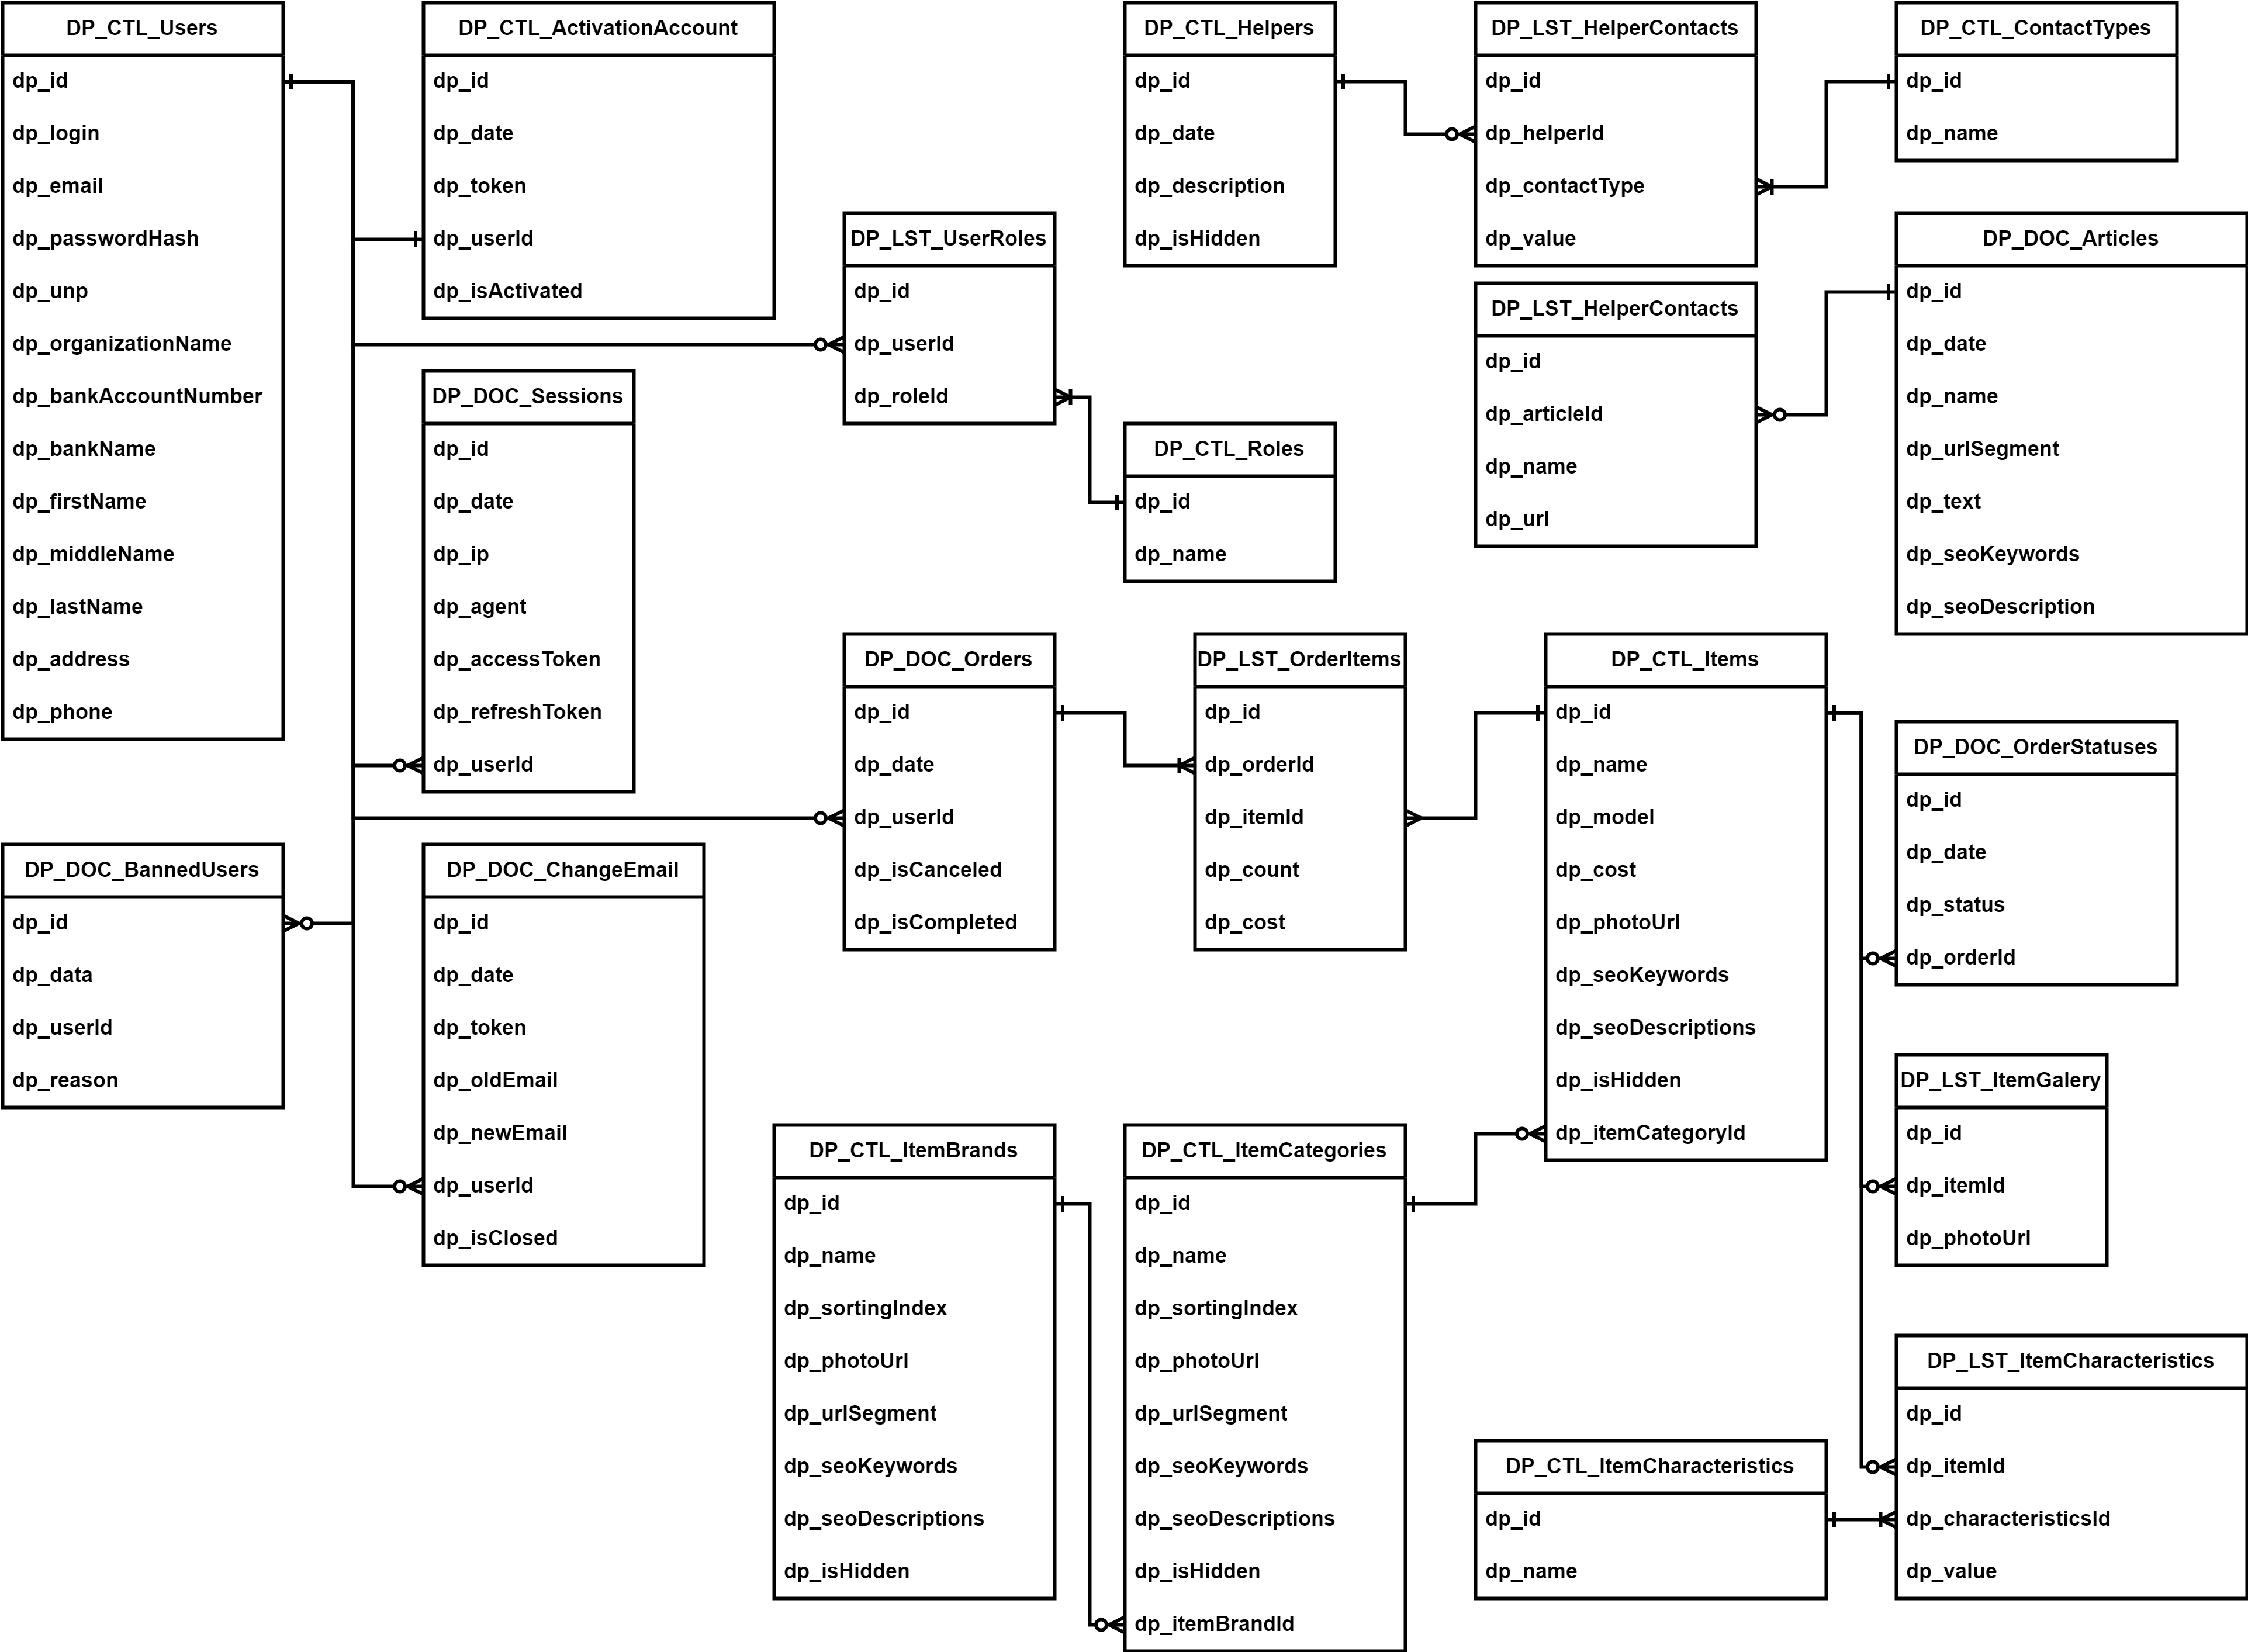
\includegraphics[angle=90, width=18cm]
    {images/db/db.png}

    \caption{Логическая модель}

    \label{fig:db_logic_model}
\end{figure}
